% Figures from the saved study, package revision 2026-10-24.
% Example paths are relative to the LaTeX project root if the repository root is that project root.
% Adjust \graphicspath if the TeX project lives elsewhere.

\begin{figure}[htbp]
  \centering
  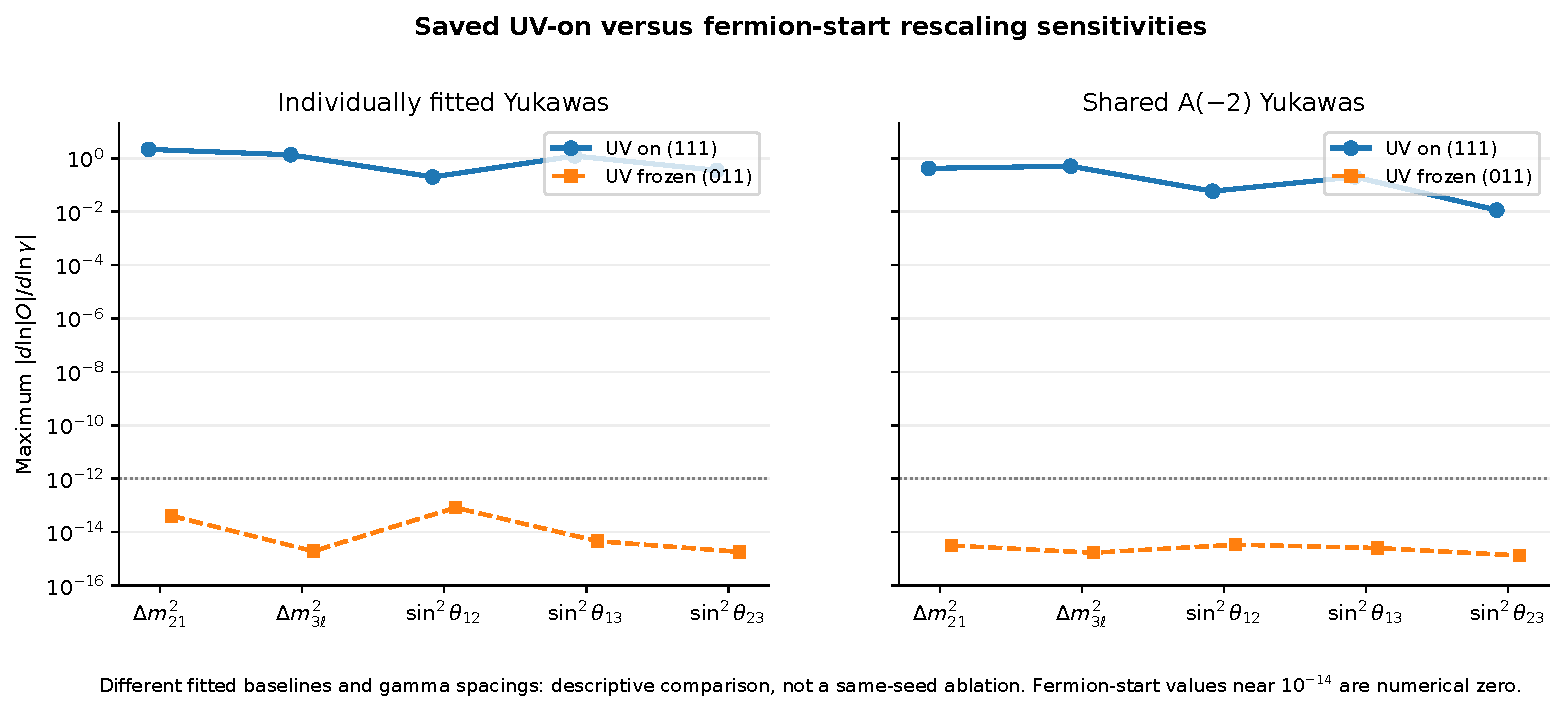
\includegraphics[width=\textwidth]{Reports/output/thesis_assets/figures/fig11_saved_uv_vs_fermion_sensitivity.pdf}
  \caption{Maximum absolute logarithmic sensitivity of the five fitted neutrino observables to the three matching-preserving coupling transformations, comparing the saved UV-running (111) and fermion-threshold-start (011) scans. Maxima are taken over all 16 model representations and three scaling directions, separately for optimised and shared-Yukawa studies. The scans use separately fitted inputs and different parameter-step sizes, so the comparison is not a controlled same-seed UV ablation; values near $10^{-14}$ reflect numerical precision.}
  \label{fig:uv_vs_fermion_saved_slopes}
\end{figure}

\begin{figure}[htbp]
  \centering
  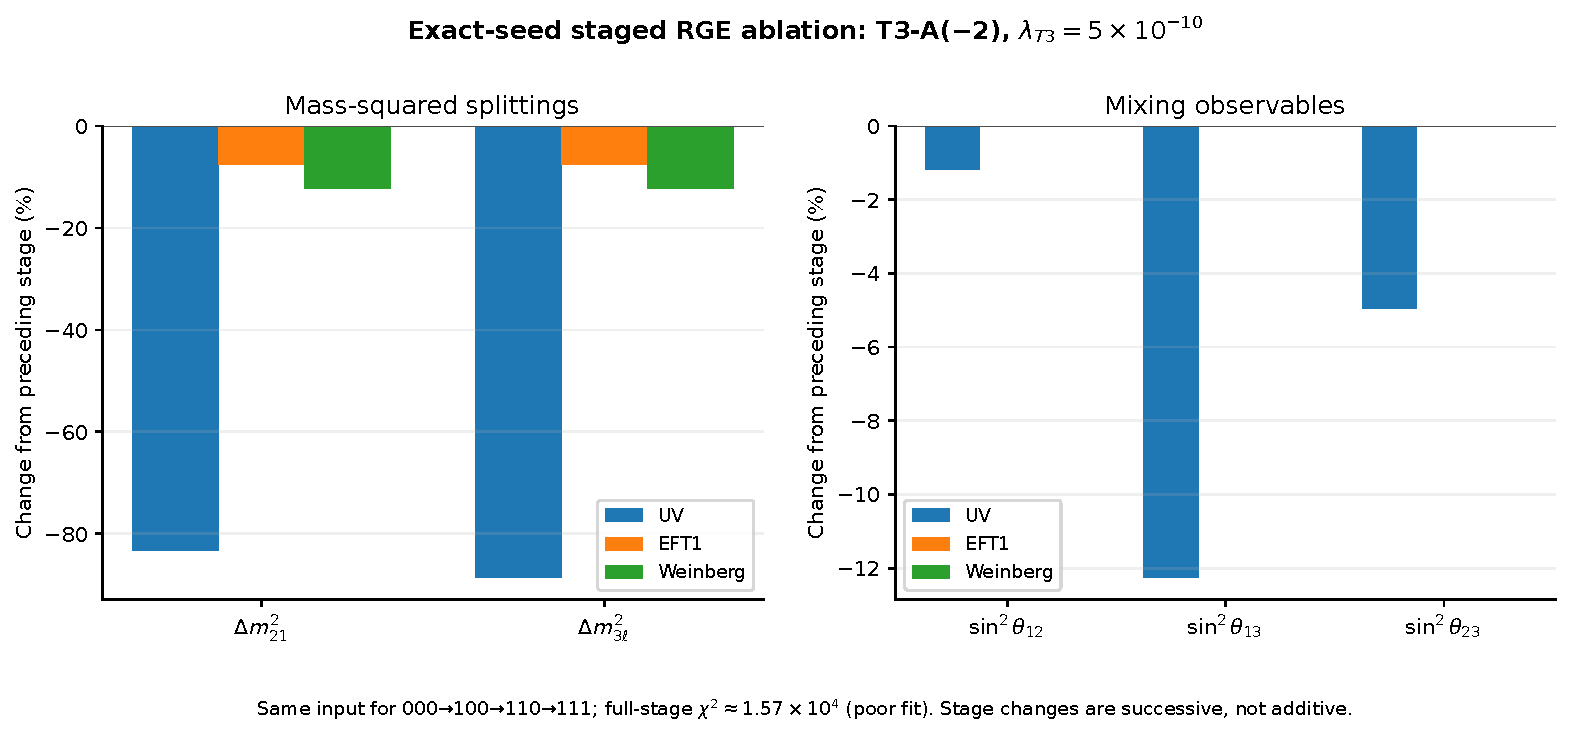
\includegraphics[width=\textwidth]{Reports/output/thesis_assets/figures/fig12_same_seed_staged_ablation.pdf}
  \caption{Successive percentage changes in mass-squared splittings and mixing observables when UV, scalar-only-EFT, and SM+Weinberg evolution are enabled in turn, using one identical T3-A($-2$) prepared seed at $\lambda_{T3}=5\times10^{-10}$. Threshold matching is retained in every configuration. The final fit has $\chi^2\simeq1.57\times10^4$, making this a diagnostic rather than a viable phenomenological benchmark. Stage percentages are not additive.}
  \label{fig:uv_exact_seed_ablation}
\end{figure}

\begin{figure}[htbp]
  \centering
  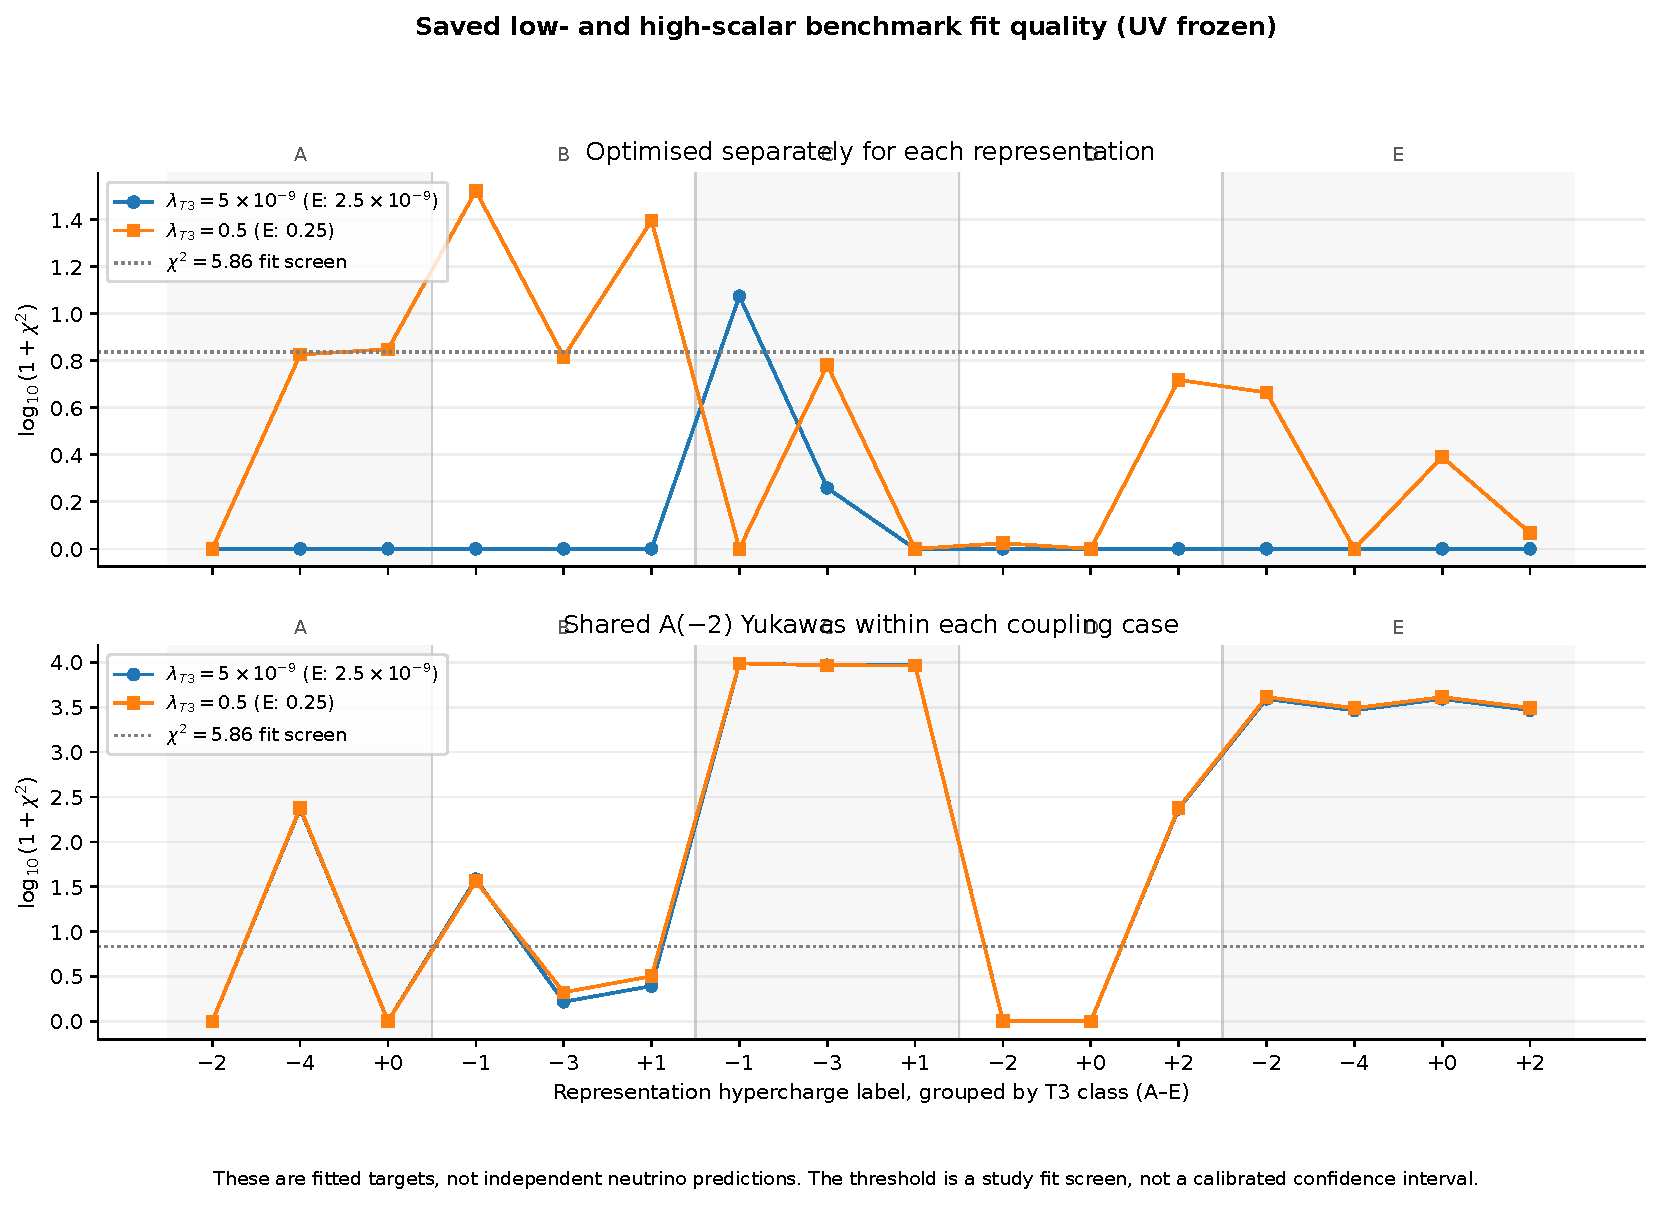
\includegraphics[width=\textwidth]{Reports/output/thesis_assets/figures/fig13_low_high_scalar_fit_quality.pdf}
  \caption{Comparison of the saved fermion-start optimised and shared-Yukawa fit qualities across 16 T3 representations for small and large $\lambda_{T3}$. The high-scalar case uses $\lambda_{T3}=0.5$ (0.25 for class E), while the low-scalar case uses $5\times10^{-9}$ ($2.5\times10^{-9}$ for class E). The dotted line denotes the study's $\chi^2=5.86$ fit-screen criterion, not a calibrated confidence threshold. Since oscillation observables are targets of these fits, fit quality is not an independent prediction.}
  \label{fig:high_scalar_fit_quality}
\end{figure}

\begin{figure}[htbp]
  \centering
  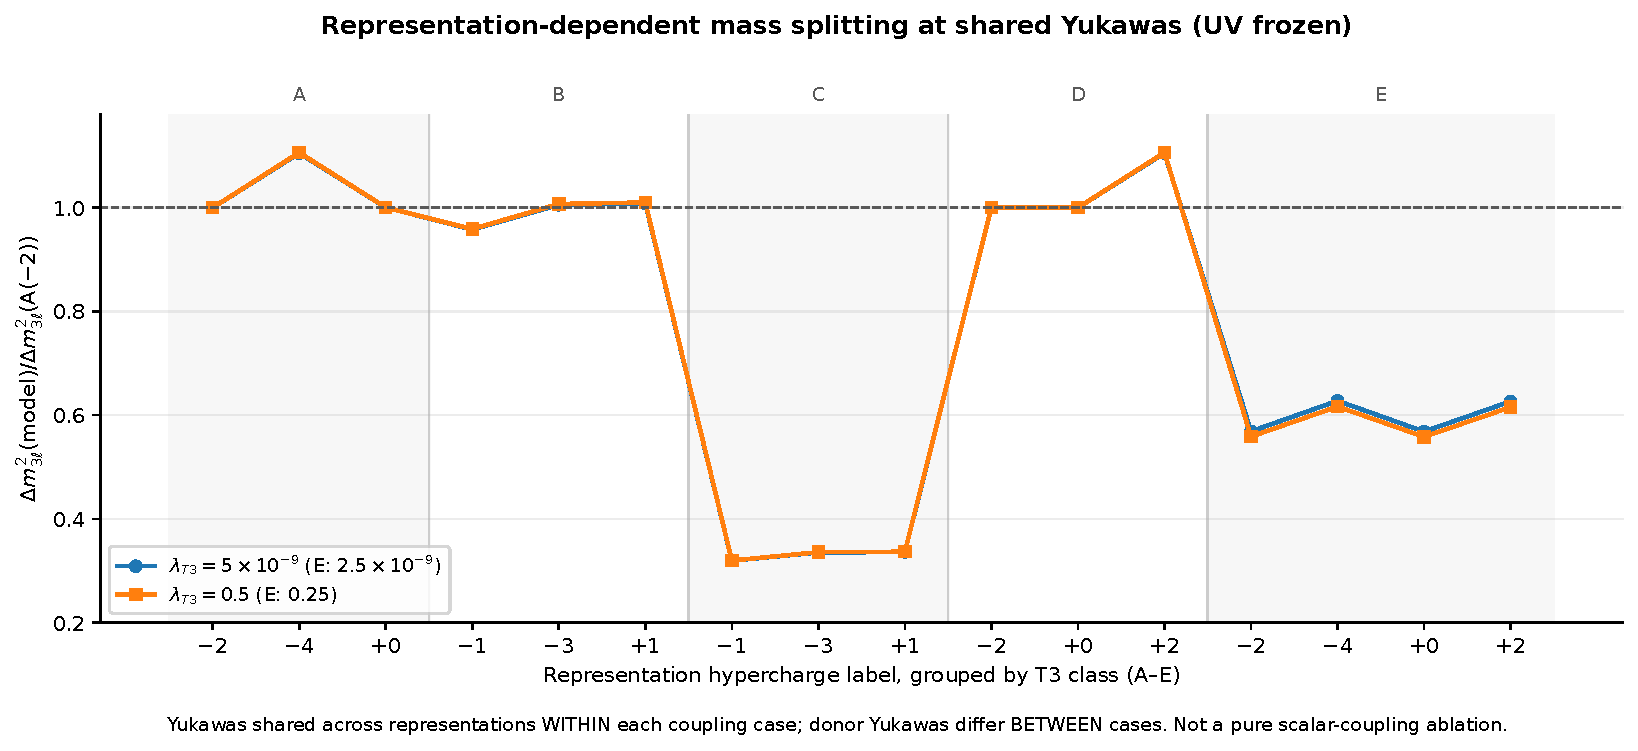
\includegraphics[width=\textwidth]{Reports/output/thesis_assets/figures/fig14_shared_yukawa_representation_effect.pdf}
  \caption{Predicted atmospheric mass-squared splitting relative to the A($-2$) reference in each of the 16 T3 representations, keeping the reference Yukawa matrices common across models within a scalar-coupling case. The persistent representation-dependent variation illustrates the impact of model-dependent matching and running coefficients. Because the fitted A($-2$) donor Yukawas differ between the two coupling cases, this plot does not isolate a fixed-input dependence on $\lambda_{T3}$.}
  \label{fig:shared_yukawa_representations}
\end{figure}
